
%% bare_conf.tex
%% V1.3
%% 2007/01/11
%% by Michael Shell
%% See:
%% http://www.michaelshell.org/
%% for current contact information.
%%
%% This is a skeleton file demonstrating the use of IEEEtran.cls
%% (requires IEEEtran.cls version 1.7 or later) with an IEEE conference paper.
%%
%% Support sites:
%% http://www.michaelshell.org/tex/ieeetran/
%% http://www.ctan.org/tex-archive/macros/latex/contrib/IEEEtran/
%% and
%% http://www.ieee.org/

%%*************************************************************************
%% Legal Notice:
%% This code is offered as-is without any warranty either expressed or
%% implied; without even the implied warranty of MERCHANTABILITY or
%% FITNESS FOR A PARTICULAR PURPOSE!
%% User assumes all risk.
%% In no event shall IEEE or any contributor to this code be liable for
%% any damages or losses, including, but not limited to, incidental,
%% consequential, or any other damages, resulting from the use or misuse
%% of any information contained here.
%%
%% All comments are the opinions of their respective authors and are not
%% necessarily endorsed by the IEEE.
%%
%% This work is distributed under the LaTeX Project Public License (LPPL)
%% ( http://www.latex-project.org/ ) version 1.3, and may be freely used,
%% distributed and modified. A copy of the LPPL, version 1.3, is included
%% in the base LaTeX documentation of all distributions of LaTeX released
%% 2003/12/01 or later.
%% Retain all contribution notices and credits.
%% ** Modified files should be clearly indicated as such, including  **
%% ** renaming them and changing author support contact information. **
%%
%% File list of work: IEEEtran.cls, IEEEtran_HOWTO.pdf, bare_adv.tex,
%%                    bare_conf.tex, bare_jrnl.tex, bare_jrnl_compsoc.tex
%%*************************************************************************

% *** Authors should verify (and, if needed, correct) their LaTeX system  ***
% *** with the testflow diagnostic prior to trusting their LaTeX platform ***
% *** with production work. IEEE's font choices can trigger bugs that do  ***
% *** not appear when using other class files.                            ***
% The testflow support page is at:
% http://www.michaelshell.org/tex/testflow/



% Note that the a4paper option is mainly intended so that authors in
% countries using A4 can easily print to A4 and see how their papers will
% look in print - the typesetting of the document will not typically be
% affected with changes in paper size (but the bottom and side margins will).
% Use the testflow package mentioned above to verify correct handling of
% both paper sizes by the user's LaTeX system.
%
% Also note that the "draftcls" or "draftclsnofoot", not "draft", option
% should be used if it is desired that the figures are to be displayed in
% draft mode.
%
\documentclass[conference]{IEEEtran}
% Add the compsoc option for Computer Society conferences.
%
% If IEEEtran.cls has not been installed into the LaTeX system files,
% manually specify the path to it like:
% \documentclass[conference]{../sty/IEEEtran}

\IEEEoverridecommandlockouts

% Turkce karakterler icin.
%\usepackage[turkish]{babel}
\usepackage[utf8]{inputenc} % Kullanılan encodinge göre utf8 yerine latin5 de yazılabilir.
\usepackage[T1]{fontenc}



% Some very useful LaTeX packages include:
% (uncomment the ones you want to load)


% *** MISC UTILITY PACKAGES ***
%
%\usepackage{ifpdf}
% Heiko Oberdiek's ifpdf.sty is very useful if you need conditional
% compilation based on whether the output is pdf or dvi.
% usage:
% \ifpdf
%   % pdf code
% \else
%   % dvi code
% \fi
% The latest version of ifpdf.sty can be obtained from:
% http://www.ctan.org/tex-archive/macros/latex/contrib/oberdiek/
% Also, note that IEEEtran.cls V1.7 and later provides a builtin
% \ifCLASSINFOpdf conditional that works the same way.
% When switching from latex to pdflatex and vice-versa, the compiler may
% have to be run twice to clear warning/error messages.






% *** CITATION PACKAGES ***
%
\usepackage{cite}
% cite.sty was written by Donald Arseneau
% V1.6 and later of IEEEtran pre-defines the format of the cite.sty package
% \cite{} output to follow that of IEEE. Loading the cite package will
% result in citation numbers being automatically sorted and properly
% "compressed/ranged". e.g., [1], [9], [2], [7], [5], [6] without using
% cite.sty will become [1], [2], [5]--[7], [9] using cite.sty. cite.sty's
% \cite will automatically add leading space, if needed. Use cite.sty's
% noadjust option (cite.sty V3.8 and later) if you want to turn this off.
% cite.sty is already installed on most LaTeX systems. Be sure and use
% version 4.0 (2003-05-27) and later if using hyperref.sty. cite.sty does
% not currently provide for hyperlinked citations.
% The latest version can be obtained at:
% http://www.ctan.org/tex-archive/macros/latex/contrib/cite/
% The documentation is contained in the cite.sty file itself.






% *** GRAPHICS RELATED PACKAGES ***
%
\ifCLASSINFOpdf
  \usepackage[pdftex]{graphicx}
  % declare the path(s) where your graphic files are
  % \graphicspath{{../pdf/}{../jpeg/}}
  % and their extensions so you won't have to specify these with
  % every instance of \includegraphics
  % \DeclareGraphicsExtensions{.pdf,.jpeg,.png}
\else
  % or other class option (dvipsone, dvipdf, if not using dvips). graphicx
  % will default to the driver specified in the system graphics.cfg if no
  % driver is specified.
  % \usepackage[dvips]{graphicx}
  % declare the path(s) where your graphic files are
  % \graphicspath{{../eps/}}
  % and their extensions so you won't have to specify these with
  % every instance of \includegraphics
  % \DeclareGraphicsExtensions{.eps}
\fi
% graphicx was written by David Carlisle and Sebastian Rahtz. It is
% required if you want graphics, photos, etc. graphicx.sty is already
% installed on most LaTeX systems. The latest version and documentation can
% be obtained at:
% http://www.ctan.org/tex-archive/macros/latex/required/graphics/
% Another good source of documentation is "Using Imported Graphics in
% LaTeX2e" by Keith Reckdahl which can be found as epslatex.ps or
% epslatex.pdf at: http://www.ctan.org/tex-archive/info/
%
% latex, and pdflatex in dvi mode, support graphics in encapsulated
% postscript (.eps) format. pdflatex in pdf mode supports graphics
% in .pdf, .jpeg, .png and .mps (metapost) formats. Users should ensure
% that all non-photo figures use a vector format (.eps, .pdf, .mps) and
% not a bitmapped formats (.jpeg, .png). IEEE frowns on bitmapped formats
% which can result in "jaggedy"/blurry rendering of lines and letters as
% well as large increases in file sizes.
%
% You can find documentation about the pdfTeX application at:
% http://www.tug.org/applications/pdftex





% *** MATH PACKAGES ***
%
\usepackage[cmex10]{amsmath}
% A popular package from the American Mathematical Society that provides
% many useful and powerful commands for dealing with mathematics. If using
% it, be sure to load this package with the cmex10 option to ensure that
% only type 1 fonts will utilized at all point sizes. Without this option,
% it is possible that some math symbols, particularly those within
% footnotes, will be rendered in bitmap form which will result in a
% document that can not be IEEE Xplore compliant!
%
% Also, note that the amsmath package sets \interdisplaylinepenalty to 10000
% thus preventing page breaks from occurring within multiline equations. Use:
%\interdisplaylinepenalty=2500
% after loading amsmath to restore such page breaks as IEEEtran.cls normally
% does. amsmath.sty is already installed on most LaTeX systems. The latest
% version and documentation can be obtained at:
% http://www.ctan.org/tex-archive/macros/latex/required/amslatex/math/





% *** SPECIALIZED LIST PACKAGES ***
%
%\usepackage{algorithmic}
% algorithmic.sty was written by Peter Williams and Rogerio Brito.
% This package provides an algorithmic environment fo describing algorithms.
% You can use the algorithmic environment in-text or within a figure
% environment to provide for a floating algorithm. Do NOT use the algorithm
% floating environment provided by algorithm.sty (by the same authors) or
% algorithm2e.sty (by Christophe Fiorio) as IEEE does not use dedicated
% algorithm float types and packages that provide these will not provide
% correct IEEE style captions. The latest version and documentation of
% algorithmic.sty can be obtained at:
% http://www.ctan.org/tex-archive/macros/latex/contrib/algorithms/
% There is also a support site at:
% http://algorithms.berlios.de/index.html
% Also of interest may be the (relatively newer and more customizable)
% algorithmicx.sty package by Szasz Janos:
% http://www.ctan.org/tex-archive/macros/latex/contrib/algorithmicx/




% *** ALIGNMENT PACKAGES ***
%
%\usepackage{array}
% Frank Mittelbach's and David Carlisle's array.sty patches and improves
% the standard LaTeX2e array and tabular environments to provide better
% appearance and additional user controls. As the default LaTeX2e table
% generation code is lacking to the point of almost being broken with
% respect to the quality of the end results, all users are strongly
% advised to use an enhanced (at the very least that provided by array.sty)
% set of table tools. array.sty is already installed on most systems. The
% latest version and documentation can be obtained at:
% http://www.ctan.org/tex-archive/macros/latex/required/tools/


%\usepackage{mdwmath}
%\usepackage{mdwtab}
% Also highly recommended is Mark Wooding's extremely powerful MDW tools,
% especially mdwmath.sty and mdwtab.sty which are used to format equations
% and tables, respectively. The MDWtools set is already installed on most
% LaTeX systems. The lastest version and documentation is available at:
% http://www.ctan.org/tex-archive/macros/latex/contrib/mdwtools/


% IEEEtran contains the IEEEeqnarray family of commands that can be used to
% generate multiline equations as well as matrices, tables, etc., of high
% quality.


%\usepackage{eqparbox}
% Also of notable interest is Scott Pakin's eqparbox package for creating
% (automatically sized) equal width boxes - aka "natural width parboxes".
% Available at:
% http://www.ctan.org/tex-archive/macros/latex/contrib/eqparbox/





% *** SUBFIGURE PACKAGES ***
%\usepackage[tight,footnotesize]{subfigure}
% subfigure.sty was written by Steven Douglas Cochran. This package makes it
% easy to put subfigures in your figures. e.g., "Figure 1a and 1b". For IEEE
% work, it is a good idea to load it with the tight package option to reduce
% the amount of white space around the subfigures. subfigure.sty is already
% installed on most LaTeX systems. The latest version and documentation can
% be obtained at:
% http://www.ctan.org/tex-archive/obsolete/macros/latex/contrib/subfigure/
% subfigure.sty has been superceeded by subfig.sty.



%\usepackage[caption=false]{caption}
%\usepackage[font=footnotesize]{subfig}
% subfig.sty, also written by Steven Douglas Cochran, is the modern
% replacement for subfigure.sty. However, subfig.sty requires and
% automatically loads Axel Sommerfeldt's caption.sty which will override
% IEEEtran.cls handling of captions and this will result in nonIEEE style
% figure/table captions. To prevent this problem, be sure and preload
% caption.sty with its "caption=false" package option. This is will preserve
% IEEEtran.cls handing of captions. Version 1.3 (2005/06/28) and later
% (recommended due to many improvements over 1.2) of subfig.sty supports
% the caption=false option directly:
%\usepackage[caption=false,font=footnotesize]{subfig}
%
% The latest version and documentation can be obtained at:
% http://www.ctan.org/tex-archive/macros/latex/contrib/subfig/
% The latest version and documentation of caption.sty can be obtained at:
% http://www.ctan.org/tex-archive/macros/latex/contrib/caption/




% *** FLOAT PACKAGES ***
%
%\usepackage{fixltx2e}
% fixltx2e, the successor to the earlier fix2col.sty, was written by
% Frank Mittelbach and David Carlisle. This package corrects a few problems
% in the LaTeX2e kernel, the most notable of which is that in current
% LaTeX2e releases, the ordering of single and double column floats is not
% guaranteed to be preserved. Thus, an unpatched LaTeX2e can allow a
% single column figure to be placed prior to an earlier double column
% figure. The latest version and documentation can be found at:
% http://www.ctan.org/tex-archive/macros/latex/base/



%\usepackage{stfloats}
% stfloats.sty was written by Sigitas Tolusis. This package gives LaTeX2e
% the ability to do double column floats at the bottom of the page as well
% as the top. (e.g., "\begin{figure*}[!b]" is not normally possible in
% LaTeX2e). It also provides a command:
%\fnbelowfloat
% to enable the placement of footnotes below bottom floats (the standard
% LaTeX2e kernel puts them above bottom floats). This is an invasive package
% which rewrites many portions of the LaTeX2e float routines. It may not work
% with other packages that modify the LaTeX2e float routines. The latest
% version and documentation can be obtained at:
% http://www.ctan.org/tex-archive/macros/latex/contrib/sttools/
% Documentation is contained in the stfloats.sty comments as well as in the
% presfull.pdf file. Do not use the stfloats baselinefloat ability as IEEE
% does not allow \baselineskip to stretch. Authors submitting work to the
% IEEE should note that IEEE rarely uses double column equations and
% that authors should try to avoid such use. Do not be tempted to use the
% cuted.sty or midfloat.sty packages (also by Sigitas Tolusis) as IEEE does
% not format its papers in such ways.





% *** PDF, URL AND HYPERLINK PACKAGES ***
%
%\usepackage{url}
% url.sty was written by Donald Arseneau. It provides better support for
% handling and breaking URLs. url.sty is already installed on most LaTeX
% systems. The latest version can be obtained at:
% http://www.ctan.org/tex-archive/macros/latex/contrib/misc/
% Read the url.sty source comments for usage information. Basically,
% \url{my_url_here}.

% *** Do not adjust lengths that control margins, column widths, etc. ***
% *** Do not use packages that alter fonts (such as pslatex).         ***
% There should be no need to do such things with IEEEtran.cls V1.6 and later.
% (Unless specifically asked to do so by the journal or conference you plan
% to submit to, of course. )
\usepackage{multirow}
\usepackage{array}
\usepackage[lofdepth,lotdepth]{subfig}
\usepackage{color}

\usepackage{amssymb}
\usepackage{booktabs}
\usepackage{multirow}
\usepackage{rotating}
\usepackage{amsmath}
\usepackage{algorithm}
\usepackage{algpseudocode}
\usepackage{lineno,hyperref}
\usepackage{graphicx}
\usepackage{pdflscape}
 \usepackage[none]{hyphenat}
% correct bad hyphenation here
%\hyphenation{op-tical net-works semi-conduc-tor}


\begin{document}


\IEEEpubid{\makebox[\columnwidth]{ 978-1-7281-2420-9/19/\$31.00
\copyright 2019 IEEE\hfill} \hspace{\columnsep}\makebox[\columnwidth]{}}

%
% paper title
% can use linebreaks \\ within to get better formatting as desired
\title{Parkinson Hastalığı Teşhisi için Yapay Arı Kolonisi Temelli Öznitelik Seçimi\\
Feature Selection Based on Artificial Bee Colony for Parkinson Disease Diagnosis}

% author names and affiliations
% use a multiple column layout for up to three different
% affiliations

\author{
	
\IEEEauthorblockN{Hasan BADEM, Duran TURKUSAGI}
\IEEEauthorblockA{Bilgisayar Mühendisliği\\
	Kahramanmaraş Sütçü İmam Üniversitesi\\
	Kahramanmaraş, Türkiye\\
	hbadem@ksu.edu.tr, duranturkusagi@gmail.com
}
\and
\IEEEauthorblockN{Abdullah CALISKAN}
	\IEEEauthorblockA{Biyomedikal Mühendisliği\\
		İskenderun Teknik Üniversitesi\\
		Hatay, Türkiye\\
		abdullah.caliskan@iste.edu.tr
}
\and
\IEEEauthorblockN{Zeynel Abidin ÇİL }
	\IEEEauthorblockA{Endüstri Mühendisliği\\
		İzmir Demokrasi Üniversitesi\\
		İzmir, Türkiye\\
		zabidin.cil@idu.edu.tr
	}

}
% conference papers do not typically use \thanks and this command
% is locked out in conference mode. If really needed, such as for
% the acknowledgment of grants, issue a \IEEEoverridecommandlockouts
% after \documentclass

% for over three affiliations, or if they all won't fit within the width
% of the page, use this alternative format:
%
% use for special paper notices
%\IEEEspecialpapernotice{(Invited Paper)}




% make the title area
\maketitle

\begin{ozet}
Parkinson hastalığının ses sinyalleri üzerinden teşhis edilebilmektedir. Ses sinyallerinden öznitelik çıkarma algoritmaları ile elde edilen veriler doğrudan sınıflandırma algoritmalarında kullanılmaktadır. Çıkarılan özniteliklerin bazıları ilgili problemi temsil etme kabiliyeti yüksek iken bazılarının düşüktür. Parkinson hastalığı teşhisinde ses sinyallerinden elde edilen özniteliklerden hangilerinin sınıflandırma başarımını artırabileceğinin tespit edilebilmesi oldukça önemlidir. Bu çalışmada bahsi geçen problemin çözümü için  Yapay Arı Kolonisi algoritması temelli öznitelik seçim yaklaşımı önerilmiştir. Önerilen yöntem, literatüre yaygın kabul gören destek vektör makinesi, K en yakın komşu, Naive Bayes ve karar ağaçları sınıflandırma yöntemleriyle karşılaştırmalı olarak analiz edilmiştir.
%\boldmath
\end{ozet}
\begin{IEEEanahtar}
Parkinson hastalığı, Öznitelik seçimi, Yapay arı kolonisi
\end{IEEEanahtar}

\begin{abstract}
Parkinson's disease can be diagnosed by the speech signals. In general, the data obtained by feature extraction algorithms from the speech signals are used in any classification algorithm. Some of the extracted features have a high ability to represent the relevant problem, while others are low. In the diagnosis of Parkinson's disease, it is very important to determine which of the extracted features from the speech signals may increase the classification performance. In this paper, Artificial Bee Colony algorithm based feature selection approach is proposed for the solution of the mentioned problem. The proposed method has been analyzed in comparison with the well-known classification methods including support vector machine, k nearest neighbor, Naive Bayesian, decision tree.

%\boldmath
\end{abstract}
\begin{IEEEkeywords}
Parkinson disease, Feature selection, Artificial bee colony
\end{IEEEkeywords}

% IEEEtran.cls defaults to using nonbold math in the Abstract.
% This preserves the distinction between vectors and scalars. However,
% if the conference you are submitting to favors bold math in the abstract,
% then you can use LaTeX's standard command \boldmath at the very start
% of the abstract to achieve this. Many IEEE journals/conferences frown on
% math in the abstract anyway.

% no keywords

% For peer review papers, you can put extra information on the cover
% page as needed:
% \ifCLASSOPTIONpeerreview
% \begin{center} \bfseries EDICS Category: 3-BBND \end{center}
% \fi
%
% For peerreview papers, this IEEEtran command inserts a page break and
% creates the second title. It will be ignored for other modes.
\IEEEpeerreviewmaketitle

\IEEEpubidadjcol

\section{GİRİŞ}

Parkinson, yaşlılık dönemimde Alzheimer hastalığından sonra görülen en yaygın hastalıktır \cite{deo2015machine}. Parkinson hastalığının, mevcut yöntemlerle tamamen tedavi edilememektedir. Fakat, hastalığın erken döneminde teşhisi ve takibi hastanın yaşam konforunun artırılmasında önemli rol oynamaktadır. Parkinson hastalarının fiziksel hareketlerinde yavaşlama, kas kontrol kaybı, uzuvlarda titreme ve konuşma bozukları vb. karakteristik belirtiler bulunmaktadır \cite{SAKAR2019255,cakmur2011parkinson}. Bahsi geçen belirtiler tam olarak gözlenmeden erken tanı döneminde teşhis edilebilmesi, yaşam konforunun artırılmasında fayda sağlayacaktır. Erken tanı döneminde, hastaların konuşma bozukluklarından hastalığın teşhisi ve ilerlemesinin takip edilmesi üzerine yapılan pek çok çalışma literatürde bulunmaktadır \cite{guruler2017novel,peker2016decision}.

Parkinson hastalığını, konuşma bozukluğundan tanımlamak özenle gerçekleştirilmesi gereken zorlu bir takım süreçleri gerektirmektedir \cite{caliskan2017diagnosis,ngumuh524658,gunduz2019deep}. Bu süreçte, öncelikle ses sinyalleri bazı filtreleme teknikleriyle gürültüden arındırılmalıdır. Sonrasında gürültüden arındırılan ses sinyalleri üzerinden parkinson hastalığını en iyi biçimde temsil edebilecek özniteliklerin elde edilmesi gerekmektedir. Daha sonra elde edilen öznitelikler kullanılarak uygun bir sınıflandırma algoritmasıyla ile hastalık teşhis edilir \cite{deo2015machine}. Bu süreçte, problemi temsil edebilecek özniteliklere karar verildikten sonra, doğrudan tüm öznitelikler kullanılmaktadır. Fakat, hangi öznitelik çıkarma yöntemi kullanılırsa kullanılsın, bazı öznitelik vektörlerinin diğerlerine göre baskın olabileceği veya bazı öznitelik vektörlerinin hastalık teşhisinde sonuca fazla katkı sağlamayabileceği durumu ihmal edilmektedir. Bahsedilen bu sınırlılığın ortadan kaldırabilmesi adına, elde edilen özniteliklerden hangilerinin problemin çözümünde daha etkin olduğunun karar verilebilmesi süreci bir optimizasyon problemi olarak tanımlanabilir.

Literatürde, bir fonksiyonun optimizasyon için sunulan pek çok yöntem bulunmaktadır. Fakat, bu yöntemlerden Parçacık Sürü Optimizasyon \cite{Poli2007}, Genetik Algoritma \cite{holland1989induction} ve Yapay Arı Kolonisi (Artificial Bee Colony-ABC)  \cite{karaboga2005idea} küresel en iyi çözümü bulmada etkin sonuç üretmektedir. ABC Algoritması, test fonksiyonları üzerindeki başarısı dikkate alındığında, nispeten daha etkin bir algoritma olduğu belirtilmektedir \cite{HANCER2018462,BADEM2018826}.

Bu çalışmada, Parkinson hastalığının teşhisinde ses sinyalleri üzerinden çeşitli yöntemlerle elde edilen özniteliklerden etkin olanların, ABC algoritması ile seçilmesi amaçlanmaktadır. Ayrıca önerilen yaklaşımla seçilen özniteliklerin sınıflandırma sürecinde, literatürde kabul gören Destek Vektör Makinesi (Support Vector Machine, SVM), K-en Yakın Komşu (K-nearest neighbor-KNN) algoritması, Karar Ağaçları (Decision Tree, DT) ve Naive Bayes (NB) sınıflandırıcıların kullanılan veri setindeki performansının değerlendirilmesi amaçlanmaktadır. 

Çalışmanın ikinci bölümünde, önerilen yöntem ve karşılaştırma ölçütleri sunulmaktadır. Daha sonra, deneysel sonuçlar verilmektedir. Çalışma sonuç bölümü ile sonlandırılmaktadır.

\section{YÖNTEM}

Parkinson hastalığı teşhisi sürecinde, Şekil \ref{fig:GPHTS}'de görülen genel yaklaşım uygulanmaktadır. Bu yaklaşımda, ses sinyalleri ham veri olarak kullanılmaktadır. Elde edilen ses sinyallerinden gürültülerin filtrelenme süreci ön işlemdir \cite{ngumuh542973}. Filtrelenmiş veriden çeşitli öznitelik çıkarma algoritmalarıyla, problemi temsil edebilecek veri oluşturulmaktadır. Elde edilen bu veriler bir sınıflandırma algoritması ile hastalık teşhisi yapılmaktadır. Fakat bu genel yaklaşımda, öznitelik çıkarma algoritmalarından elde edilen verideki bazı vektörlerin probleme özgü olarak anlamlı yada anlamsız olduğuna bakılmaksızın kullanılmaktadır. Bu durum hastalık teşhisinde, başarıyı oldukça etkilemektedir. 
%
\begin{figure}[]%
	\centering%
	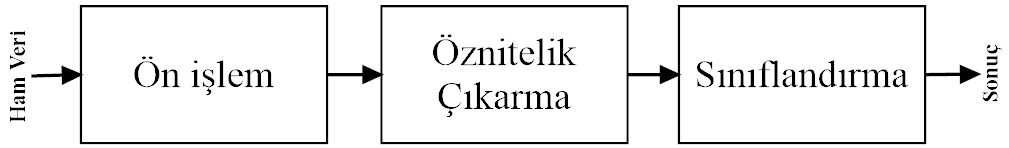
\includegraphics[width=8cm]{figures/GenelYontem.png}\\
	\caption{Genel Parkinson Hastalığı Teşhis Süreci}%
	\label{fig:GPHTS}%
\end{figure}
%
Bu çalışmada, parkinson hastalığı teşhisi sürecinde bahsi geçen problemin ortadan kaldırılması adına ABC algoritması temelli öznitelik seçme yaklaşımı önerilmektedir. Önerilen yöntemin genel yaklaşımdaki geliştirilmiş blok diyagramı Şekil \ref{fig:OPHTS}'de görülmektedir. Önerilen yöntem aşağıda alt bölümler halinde sunulmaktadır.
%
\begin{figure}[]%
	\centering%
	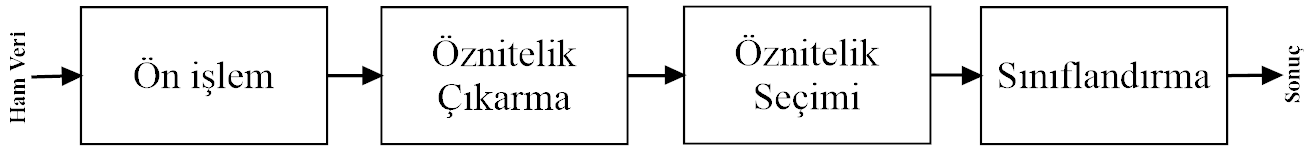
\includegraphics[width=8cm]{figures/OnerilenYontem.png}\\
	\caption{Önerilen Parkinson Hastalığı Teşhis Süreci}%
	\label{fig:OPHTS}%
\end{figure}

\subsection{Yapay Arı Kolonisi Optimizasyon Algoritması}

ABC algoritması, bal arılarının yiyecek arama sürecinde göstermiş oldukları zeki davranışı modelleyen bir optimizasyon algoritmasıdır. Bu zeki yiyecek arama süreci; görevli, gözcü ve kâşif arı olmak üzere 3 arı türü ile gerçekleştirilmektedir \cite{karaboga2005idea}.

Görevli arılar, daha önce keşfedilmiş besin kaynakları civarında araştırma yapar ve sorumlu olduğu kaynaktan besin taşımaktadır. Görevli arılar kovana döndüklerinde, sorumlu olduğu besin kaynağının yeri ve nektar kalitesi hakkında gözcü arılara titreşim dansı üzerinden bilgi aktarır. Gözcü arılar ise, izlemiş oldukları danslar elde ettikleri bilgilere göre bir besin kaynağı seçer ve araştırma işlemlerini seçmiş olduğu kaynak üzerinden gerçekleştirmektedir. Görevli arılar, sorumlu oldukları besin kaynağı tükenmiş yada kalitesi yetersiz olursa araştırmalarına kâşif arı olarak devam etmektedir. Kâşif arılar ise, rastgele bir alternatif besin kaynağı araştırmaktadır \cite{karaboga2007powerful,karaboga2009comparative,aslan2019time,gao2012modified,zhu2010gbest}.

Bal arılarının yukarıda bahsedilen sürü zekasını modelleyen ABC algoritması, Derviş KARABOĞA tarafından literatüre sunulmuştur \cite{karaboga2005idea}. ABC algoritmasında her bir besin kaynağı, bir aday çözüme karşılık gelmektedir. Aynı zamanda besin kaynaklarının nektar miktarı, aday çözümün uygunluk değerine olarak tanımlanmaktadır. En iyi çözümü araştırma sürecinde tüm arı türleri iteratif fazlar halinde araştırma yapmaktadır \cite{karaboga2007powerful,karaboga2009comparative,aslan2019time,gao2012modified,zhu2010gbest}.

%\begin{algorithm}[t]
%	\scriptsize
%	\caption{Yapay Arı Kolonisi Algoritmasının Temel Adımları}\label{alFundamentalStepsofABC}
%	\algrenewcommand\algorithmicrepeat{\textbf{Repeat}}
%	\algrenewcommand\algorithmicuntil{\textbf{Until} maksimum değerlendirme sayısı }
%	\algsetblockdefx[Initialization]{Initialization}{End}{2}{0.5cm}{\textbf{Başlangıç:}}{End}
%	\algsetblockdefx[Name]{Employed}{End}{1}{0.5cm}{\textbf{Görevli Arı Fazı:}}{End}
%	\algsetblockdefx[Name]{Onlooker}{End}{2}{0.5cm}{\textbf{Gözcü Arı Fazı:}}{End}
%	\algsetblockdefx[Name]{Scout}{End}{2}{0.5cm}{\textbf{Kâşif Arı Fazı:}}{End}
%	\begin{algorithmic}[1]
%		\Initialization
%		\State Kontrol parametrelerini belirle.
%		\State Tüm arıları Kâşif arı olarak besin kaynaklarına gönder.
%		\Repeat
%		\Employed
%		\State Tüm görevli arıları sorumlu oldukları besin kaynakları civarında yeni kaynaklar bulmak için gönder.
%		\Onlooker
%		\State Tüm besin kaynaklarının olasılık değerleri hesapla.
%		\State Besin kaynaklarının olasılık değerlerine göre, tüm gözcü arıları seçilen besin kaynakları civarında araştırma yapmak üzere gönder.
%		\Scout
%		\State Terk edilecek besin kaynağını belirle.
%		\State Terk edilecek besin kaynağından sorumlu görevli arıyı kâşif arı olarak gönder.
%		\State \textbf{En iyi besin kaynağını sakla.}
%		\Until
%	\end{algorithmic}
%\end{algorithm}

ABC algoritması, $D$ adet rastgele değerlerden oluşan $SN$ farklı besin kaynağı oluşturularak başlatılır \cite{karaboga2007powerful,karaboga2009comparative}. Bu işlem denklem \ref{eqInitialFoodSourceCreation}'de tanımlanmaktadır.
%
\begin{equation}
\label{eqInitialFoodSourceCreation}
x_{ij}=x_j^{min}+rand(0,1)(x_j^{max}-x_j^{min})
\end{equation}
%
burada; $x_{ij}$, $i$. çözümün $j$. parametresine karşılık gelmektedir. $x_{jmin}$ ve $x_{jmax}$ ise $j$. parametrenin alt ve üst sınır değerleridir \cite{karaboga2007powerful,karaboga2009comparative}.

Görevli arılar, sorumlu olduğu ve rastgele seçilen bir besin kaynağının bilgilerini kullanarak, yeni bir çözüm araştırmaya çalışır. Bu süreç aşağıdaki denklem ile modellenmiştir \cite{karaboga2007powerful,karaboga2009comparative};
%
\begin{equation}
\label{eqCandidateFoodSourceCreation}
v_{ij}=x_{ij}+\phi_{ij}(x_{ij}-x_{kj})
\end{equation}
%
burada, $k$ ve $j$ indeksleri rastgele seçilen değerlerdir. Elde edilen yeni çözümün uygunluk değeri, var olan çözümden daha kaliteli ise, görevli arı yeni çözüm ile güncellenmektedir. Tüm görevli arılar araştırma süreçlerini tamamladıktan sonra, sorumlu oldukları besin kaynaklarının kalite bilgisini gözcü arılar ile paylaşmaktadır. Her bir gözcü arı, var olan çözümlerin olasılık değerine göre, bir çözüm seçer ve görevli arı gibi denklem \ref{eqCandidateFoodSourceCreation} üzerinden aday bir çözüm üretmektedir \cite{karaboga2007powerful,karaboga2009comparative}. Besin kaynaklarının olasılık değerleri aşağıdaki denklem ile hesaplanmaktadır:
%
\begin{equation}
\label{eqProbabilityCalculation}
p_i=\frac{{fitness}_i}{\sum_{j=1}^{SN}{fitness}_j}
\end{equation}
%
Meta-sezgisel algoritmalarının araştırma sürecinde, keşif ve tüketimin işlemleri arasında bir denge olmak zorundadır. ABC algoritmasında bu denge \textit{limit} adı verilen bir kontrol parametresi ile sağlanmaktadır. Bu parametre ile besin kaynaklarının denenme sayısı kontrol edilir. ABC algoritmasının her çevriminde, \textit{limit} değerini en çok geçen besin kaynağı terk edilir ve sorumlu görevli arı, kaşif arı olarak aday bir çözüm üretmektedir. $limit$ parametresi literatürde genellikle aşağıdaki denklem üzerinden belirlenir \cite{karaboga2007powerful,karaboga2009comparative}.
%
\begin{equation}
\label{equation:LimitCalculation}
limit=\lceil a \times SN \times D \rceil \:
\end{equation}

\subsection{Öznitelik Seçimi}

Öznitelik seçim işlemi bir optimizasyon problemi olarak tasarlandığında, veri setinde çözümü temsil kabiliyeti yüksek öznitelik vektörlerinin bulunması amaçlanmaktadır. Dolayısı ile veri setindeki problemi temsil gücü zayıf olan öznitelik vektörlerinin veri setinden çıkarılarak geliştirilen sınıflandırma modelinin doğruluk değerini yükseltilmeye çalışılmaktadır. 

Parkinson hastalığı teşhisinde kullanılacak herhangi bir veri setindeki her bir $X_i$ giriş vektörüne karşılık bir çıkış $Y_i$ etiketine sahiptir. Bu çalışmada kullanılan veri setinde, $240$ örneklem ve $46$ adet öznitelik bulunmaktadır. Veri setindeki $46$ adet öznitelikten Parkinson hastalığının ses sinyalleri üzerinden teşhis edilebilmesinde, daha etkin olduğunun belirlenmesinde ABC temelli öznitelik seçimi gerçekleştirilmiştir.

ABC temelli öznitelik seçiminde, aday her bir çözümün uygunluk değeri KNN sınıflandırma algoritması ile $10$ kat çapraz doğrulama tekniği kullanarak hesaplanmıştır. Şekil \ref{fig:RepFoods}-a'da görüldüğü üzere ABC algoritmasının başlangıç aşamasında; her bir besin kaynağı için araştırma yaparken problemin temsilinde kullanılabilecek her bir öznitelik vektörünü temsilen $(0,1)$ arasında rastgele reel sayılar oluşturulmuştur. Bu reel değerler üzerinden araştırma yapılırken, besin kaynağının uygunluk değeri hesaplanırken önceden belirlenen bir eşik değerine göre $0$ veya $1$ değerinde seçim vektörü oluşturulmaktadır. Bu durum Şekil \ref{fig:RepFoods}-b'de görülmektedir.
%
\begin{figure}[!h]
	\centering%
	%\scriptsize
	\begin{center}
		\begin{tabular}{cc}%
			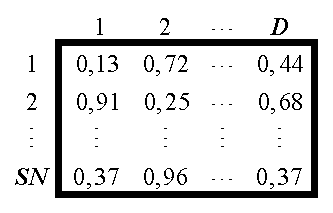
\includegraphics[height=2.5cm]{figures/m1.pdf}&%
			
			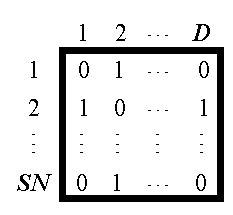
\includegraphics[height=2.6cm]{figures/m2.pdf}\\%
			(a) Araştırma&  (b) Uygunluk \\%
		\end{tabular}%
	\end{center}
	\caption{ABC algoritmasında besin kaynaklarının temsili}%
	\label{fig:RepFoods}
\end{figure}
%
ABC algoritmasında, çözüm uzayını temsil eden her bir besin kaynağının parametre sayısı ($D$), Parkinson hastalığı teşhisi için oluşturulan veri setindeki öznitelik sayısına eşittir. Öznitelik seçim vektöründe kullanılan eşik değeri $0.5$ alınmıştır. ABC algoritması temelli öznitelik seçim sürecinde, besin kaynağı sayısı; $10, 20, 40, 50$ ve $100$ alınmıştır. Ayrıca, çevrim sayısı ise $10, 100, 500$ ve $1000$ alınmıştır. Bu kontrol parametrelerinin her bir kombinasyonu için önerilen algoritma çalıştırılmıştır. En yüksek doğruluk oranını, besin kaynağı $20$ ve çevrim sayısı $1000$ olan kombinasyon vermiştir. Deneysel sonuçlar bu kombinasyon üzerinden elde edilmiştir.

\section{DENEYSEL SONUÇLAR ve TARTIŞMA}

Deneysel sonuçları elde edebilmek için UCI makine öğrenmesi deposunda 2019 yılında paylaşılmış olan "Akustik Özelliklere Sahip Parkinson Veri Kümesi" veri seti \cite{naranjo2016addressing,naranjo2017two} kullanılmıştır. Makine öğrenmesi yöntemlerini karşılaştırabilmek için 10 kat çapraz doğrulama tekniği ile 30 farklı koşma gerçekleştirilmiştir. Elde edilen sonuçlar, 2.0 GHz Intel i7-4510 işlemcili ve 12 GB RAM belleğe sahip sistem üzerinden elde edilmiştir.

Bu bölümde, öncelikle kullanılan veri setinden bahsedilmekte, daha sonra karşılaştırmalı olarak elde edilen simülasyon sonuçları sunulmaktadır.

\subsection{Akustik Özelliklere Sahip Parkinson Veri Kümesi veri seti}

Akustik Özelliklere Sahip Parkinson Veri Kümesi (Parkinson Dataset with replicated acoustic features-PDRAF) veri setinin geliştirilme amacı, bireylerin ses kayıtları üzerinden hastalığın tespit edilebilmesi için  klinik uzman sistem geliştirmektir. Bu amaç için bireylerin ses kayıtlarından özellikler çıkararak  örüntü tanıma için gelişmiş bir istatistiksel yaklaşım göz önünde bulunduran  veri seti oluşturulmuştur \cite{naranjo2016addressing}. PDRAF veri seti 2019 yılında UCI Makine öğrenmesi \cite{UCI} deposundan paylaşılmıştır. Literatürde ses sinyalleri üzerinden Parkinson hastalığının teşhis edilebilmesi için birkaç veri seti daha bulunmaktadır. PDRAF  diğer veri setleri arasında, bu çalışmanın yapıldığı tarihe göre en güncel veri setidir. PDRAF veri seti için kullanılan Parkinson Hastalığına sahip hastalar İspanya Ekstremadura Bölgesel Parkinson Hastalığı Derneği üyelerinden seçilmiştir\cite{naranjo2016addressing}. PDRAF veri seti oluşturulurken çalışmaya $50$ yaşından büyük $80$ kişi katılmıştır. Hastaların $40$'ı sağlıklı: $22$ erkek ($\% 55$) ve $18$ kadın ($\% 45$) ve $40$'ı PD: $27$ erkek ($\% 67,5$) ve $13$ kadın ($\% 32,5$) tarafından oluşmaktadır. Ortalama yaş, kontrol grubu için $66,38$ ve PD'li kişilerde $69,58$ dir.

Ses kayıtları, deneklere  "a"  ünlü harfinin rahat ve yüksek sesle en az 5 saniye ve bir nefeste söyletilmesiyle elde edilmiştir. Veri toplama süreci, kişi başına üç kez tekrarlanmıştır \cite{naranjo2016addressing}. Dijital kayıt, Audacity yazılımı (sürüm 2.0.5) kullanılarak $44.1$ KHz örnekleme hızında ve $16$ bit/örnek çözünürlükte yapılmıştır \cite{naranjo2016addressing}.

\subsection{Simülasyon Sonuçları}

ABC algoritmasıyla elde edilen en iyi öznitelik vektörleri, tüm karşılaştırma yöntemlerinde kullanılarak deneysel sonuçlar elde edilmiştir. Parkinson hastalığının teşhis edilebilmesi için, PDRAF veri seti üzerinden SVM, KNN, DT ve NB sınıflandırıcıları 10 kat çapraz doğrulama tekniği ile $30$ farklı koşma gerçekleştirilmiştir. Gerçekleştirilen bu simülasyonlardan, $30$ farklı koşmanın \textit{acc, AUC, sn, sp, f, p} değerleri kaydedilmiştir. Bu değerlerin ortalama ve standart sapmaları Tablo \ref{tbl:AccAuc}, Tablo \ref{tbl:SnSp} ve Tablo \ref{tbl:PF}’te verilmiştir.
%
\begin{table}[h]
	\centering
	\begin{tabular}{|l|c|c|c|c|}
		\hline
		& \multicolumn{2}{c|}{\textit{\textbf{acc}}}  & \multicolumn{2}{c|}{\textit{\textbf{AUC}}}     \\ \hline
		& \textbf{Ortalama} & \textbf{Standart Sapma} & \textbf{Ortalama}    & \textbf{Standart Sapma} \\ \hline
		\textbf{SVM} & 73,347       & \textbf{0,850}    & 71,142         & 2,206             \\ \hline
		\textbf{KNN} & \textbf{82,375}   & 1,248             & \textbf{82,086} & \textbf{2,165}    \\ \hline
		\textbf{DT}  & 67,986       & 2,237             & 67,410          & 2,488             \\ \hline
		\textbf{NB}  & 61,263       & 1,196             & 64,375          & 2,685              \\ \hline
	\end{tabular}
	\caption{SVM, KNN, DT ve NB sınıflandırıcılarının $30$ koşmadaki \textit{acc ve AUC} ölçütlerinin ortalama ve standart sapma değerleri}
	\label{tbl:AccAuc}
\end{table}
%
\begin{table}[h]
	\centering
	\begin{tabular}{|l|c|c|c|c|}
		\hline
		\multicolumn{1}{|c|}{} & \multicolumn{2}{c|}{\textit{\textbf{sn}}}      & \multicolumn{2}{c|}{\textit{\textbf{sp}}}      \\ \hline
		\multicolumn{1}{|c|}{} & \textbf{Ortalama}    & \textbf{Standart Sapma} & \textbf{Ortalama}    & \textbf{Standart Sapma} \\ \hline
		\textbf{SVM}           & 61,047          & 2,024             & 81,630          & \textbf{1,190}    \\ \hline
		\textbf{KNN}           & 78,296         & 2,069            & \textbf{85,208} & 1,521            \\ \hline
		\textbf{DT}            & 61,515          & 3,390              & 72,604           & 2,841            \\ \hline
		\textbf{NB}            & \textbf{78,451} & \textbf{1,649}    & 49,733         & 1,769             \\ \hline
	\end{tabular}
	\caption{SVM, KNN, DT ve NB sınıflandırıcılarının 30 koşmadaki \textit{sn ve sp} ölçütlerinin ortalama ve standart sapma değerleri}
	\label{tbl:SnSp}
\end{table}
%
\begin{table}[h]
	\centering
	\begin{tabular}{|l|c|c|c|c|}
		\hline
		\multicolumn{1}{|c|}{\textbf{}} & \multicolumn{2}{c|}{\textit{\textbf{f}}}       & \multicolumn{2}{c|}{\textit{\textbf{p}}}       \\ \hline
		\multicolumn{1}{|c|}{\textbf{}} & \textbf{Ortalama}    & \textbf{Standart Sapma} & \textbf{Ortalama}    & \textbf{Standart Sapma} \\ \hline
		\textbf{SVM}                    & 63,385          & 1,664             & 69,095        & 2,10             \\ \hline
		\textbf{KNN}                    & \textbf{77,298} & 1,674            & \textbf{78,519} & 2,254             \\ \hline
		\textbf{DT}                     & 59,156          & 2,763            & 60,032          & 3,301             \\ \hline
		\textbf{NB}                     & 60,948         & \textbf{1,081}    & 51,368          & \textbf{1,051}    \\ \hline
	\end{tabular}
	\caption{SVM, KNN, DT ve NB sınıflandırıcılarının 30 koşmadaki \textit{f ve p} ölçütlerinin ortalama ve standart sapma değerleri}
	\label{tbl:PF}
\end{table}
%
Tablo I incelendiğinde; $82,37$ ile en yüksek ortalama doğruluk değerine KNN algoritması sahipken, daha sonra SVM algoritması ile ortalama $73,34$ doğruluk değeri elde edilmiştir. DT ve NB yöntemleri sırasıyla $67,98$; $61,26$ ortalama doğruluk değerleri elde edilmiştir. Doğruluk değerleri incelendiğinde, diğer yöntemler ile KNN arasında, KNN algoritmasının lehine önemli bir fark olduğu görülmektedir. Aynı zamanda, KNN algoritması, DT ve NB yöntemlerine göre oldukça üstün bir doğruluk değeri elde ettiği Tablo I’de görülmektedir. Sınıflandırma algoritmalarının başarılarını karşılaştırmada en önemli ölçütlerden olan \textit{AUC}  değerlerinde de KNN algoritmasının, diğer yöntemlere göre üstün bir başarı elde ettiği görülmektedir.
\textit{sn}  açısından Tablo II incelendiğinde, Parkinson hastalığına sahip bireyleri doğru olarak tespit edebilme başarımında, NB ve  KNN algoritması karşılaştırıldığında NB algoritmasının lehine bir fark olduğu görülmektedir. Aynı zamanda, NB algoritmasının, DT ve SVM algoritmalarına göre üstün bir başarı gösterdiği görülmektedir. Fakat, Parkinson hastalığı bulunmayan bireylerin doğru olarak tespit edilebilmesinde KNN sınıflandırıcısının SVM ve DT yöntemlerine göre daha başarılı olduğu görülmektedir. Aynı zamanda, KNN algoritmasının NB algoritmasına göre oldukça üstün bir başarı elde ettiği anlaşılmaktadır.

Parkinson hastalığına sahip olduğu tahmin edilen bireylerin gerçekte ne kadarının hastalığa sahip olduğunu gösteren \textit{p} ölçütüdür. Tablo 3 bu açıdan incelendiğinde; KNN sınıflandırıcısı, SVM,DT ve NB yöntemlerine göre  üstün bir başarı elde ettiği görülmektedir. \textit{f} açısından Tablo III değerlendirildiğinde ise, KNN sınıflandırıcısının, diğer yöntemlere göre üstün bir başarı elde ettiği görülmektedir.

Karşılaştırma ölçütleri genel olarak değerlendirildiğinde, KNN algoritması rakip algoritmalara göre üstünlük sağladığı anlaşılmaktadır.

\section{SONUÇ}

Bu çalışmada, Parkinson hastalığının ses sinyalleri üzerinden teşhis edilebilmesi için ABC algoritması temelli öznitelik seçim modeli önerilmiştir. Önerilen model ile elde edilen öznitelikler, geleneksel sınıflandırma yöntemlerinde karşılaştırmalı olarak test edilmiştir. Elde edilen deneysel sonuçlarda KNN algoritması ile sınıflandırma sonuçlarının daha yüksek olduğu ortaya çıkmıştır. Önerilen yöntem ile Parkinson hastalığının teşhisinde kullanılabilecek özniteliklerden hangilerinin problemi temsil kabiliyetinin daha yüksek olduğu belirlenebilmektedir. Bu açıdan önerilen yöntem ile hastalığının teşhisinde kullanılabilecek tüm sınıflandırma algoritmalarının başarımını artırabilir.

Parkinson hastalığının konuşma bozuklukları dışında hareket bozuklukları, koordinasyon zayıflaması vb. birçok belirtisi daha bulunmaktadır. Bu belirtileri de kapsayacak yeni özniteliklere sahip yeni veri setlerinde de önerilen yöntemin başarımının araştırılması hastalık teşhisinde doğruluk oranını artırabileceği düşünülebilir. Bu nedenle, bu alandaki gerçekleştirilebilecek yeni araştırmalar hasta konforu açısından önem arz etmektedir.


% An example of a floating figure using the graphicx package.
% Note that \label must occur AFTER (or within) \caption.
% For figures, \caption should occur after the \includegraphics.
% Note that IEEEtran v1.7 and later has special internal code that
% is designed to preserve the operation of \label within \caption
% even when the captionsoff option is in effect. However, because
% of issues like this, it may be the safest practice to put all your
% \label just after \caption rather than within \caption{}.
%
% Reminder: the "draftcls" or "draftclsnofoot", not "draft", class
% option should be used if it is desired that the figures are to be
% displayed while in draft mode.
%
%\begin{figure}[!t]
%\centering
%\includegraphics[width=2.5in]{myfigure}
% where an .eps filename suffix will be assumed under latex,
% and a .pdf suffix will be assumed for pdflatex; or what has been declared
% via \DeclareGraphicsExtensions.
%\caption{Simulation Results}
%\label{fig_sim}
%\end{figure}

% Note that IEEE typically puts floats only at the top, even when this
% results in a large percentage of a column being occupied by floats.

% An example of a double column floating figure using two subfigures.
% (The subfig.sty package must be loaded for this to work.)
% The subfigure \label commands are set within each subfloat command, the
% \label for the overall figure must come after \caption.
% \hfil must be used as a separator to get equal spacing.
% The subfigure.sty package works much the same way, except \subfigure is
% used instead of \subfloat.
%
%\begin{figure*}[!t]
%\centerline{\subfloat[Case I]\includegraphics[width=2.5in]{subfigcase1}%
%\label{fig_first_case}}
%\hfil
%\subfloat[Case II]{\includegraphics[width=2.5in]{subfigcase2}%
%\label{fig_second_case}}}
%\caption{Simulation results}
%\label{fig_sim}
%\end{figure*}
%
% Note that often IEEE papers with subfigures do not employ subfigure
% captions (using the optional argument to \subfloat), but instead will
% reference/describe all of them (a), (b), etc., within the main caption.


% An example of a floating table. Note that, for IEEE style tables, the
% \caption command should come BEFORE the table. Table text will default to
% \footnotesize as IEEE normally uses this smaller font for tables.
% The \label must come after \caption as always.
%
%\begin{table}[!t]
%% increase table row spacing, adjust to taste
%\renewcommand{\arraystretch}{1.3}
% if using array.sty, it might be a good idea to tweak the value of
% \extrarowheight as needed to properly center the text within the cells
%\caption{An Example of a Table}
%\label{table_example}
%\centering
%% Some packages, such as MDW tools, offer better commands for making tables
%% than the plain LaTeX2e tabular which is used here.
%\begin{tabular}{|c||c|}
%\hline
%One & Two\\
%\hline
%Three & Four\\
%\hline
%\end{tabular}
%\end{table}


% Note that IEEE does not put floats in the very first column - or typically
% anywhere on the first page for that matter. Also, in-text middle ("here")
% positioning is not used. Most IEEE journals/conferences use top floats
% exclusively. Note that, LaTeX2e, unlike IEEE journals/conferences, places
% footnotes above bottom floats. This can be corrected via the \fnbelowfloat
% command of the stfloats package.


% use section* for acknowledgement
%\section*{TEŞEKKÜR}
%Yazarın teşekkür etmek istediği kurum yada kişiler burada belirtilecek.

% trigger a \newpage just before the given reference
% number - used to balance the columns on the last page
% adjust value as needed - may need to be readjusted if
% the document is modified later
%\IEEEtriggeratref{8}
% The "triggered" command can be changed if desired:
%\IEEEtriggercmd{\enlargethispage{-5in}}

% references section

% can use a bibliography generated by BibTeX as a .bbl file
% BibTeX documentation can be easily obtained at:
% http://www.ctan.org/tex-archive/biblio/bibtex/contrib/doc/
% The IEEEtran BibTeX style support page is at:
% http://www.michaelshell.org/tex/ieeetran/bibtex/
%\bibliographystyle{IEEEtran}
% argument is your BibTeX string definitions and bibliography database(s)
%\bibliography{IEEEabrv,../bib/paper}
%
% <OR> manually copy in the resultant .bbl file
% set second argument of \begin to the number of references
% (used to reserve space for the reference number labels box)

\bibliographystyle{ieeetran}
\bibliography{mybibfile}







% that's all folks
\end{document}
